\documentclass[aspectratio=169,11pt]{beamer}
\usetheme{default}
\usepackage[T1]{fontenc}
\usepackage{lmodern}
\usepackage{amsmath,amssymb,bm,booktabs,graphicx}
\usepackage{pgfplots}
\pgfplotsset{compat=1.18}
\definecolor{Navy}{HTML}{173047}
\definecolor{Teal}{HTML}{007D83}
\definecolor{Grey}{HTML}{586776}
\definecolor{Light}{HTML}{DCE5EA}
\definecolor{Recorded}{HTML}{D45B55}
\definecolor{Revised}{HTML}{21865C}
\setbeamercolor{normal text}{fg=Navy,bg=white}
\setbeamercolor{frametitle}{fg=Navy,bg=white}
\setbeamercolor{structure}{fg=Teal}
\setbeamerfont{normal text}{size=\normalsize}
\setbeamerfont{frametitle}{size=\Large,series=\bfseries}
\setbeamerfont{footline}{size=\scriptsize}
\setbeamertemplate{navigation symbols}{}
\setbeamertemplate{itemize item}{\small\color{Teal}\textbullet}
\setbeamersize{text margin left=.85cm,text margin right=.85cm}
\setbeamertemplate{frametitle}{\vspace{.22cm}\insertframetitle\par\vspace{.12cm}{\color{Light}\hrule height .7pt}\vspace{.12cm}}
\setbeamertemplate{footline}{\hspace*{.85cm}\textcolor{Grey}{MAC RGB-D VIO}\hfill\textcolor{Grey}{\insertframenumber\,/\,\inserttotalframenumber}\hspace*{.85cm}\vspace{.22cm}}
\setlength{\abovedisplayskip}{8pt}
\setlength{\belowdisplayskip}{8pt}
\newcommand{\phys}[1]{\par\vspace{.15cm}{\color{Teal}\bfseries Physical meaning}\par\vspace{.07cm}#1\par}
\newcommand{\hint}[1]{\par\vspace{.16cm}{\small\color{Grey}#1\par}}
\newcommand{\src}[1]{\note{Sources and context: #1}}
\newcommand{\Exp}{\operatorname{Exp}}
\newcommand{\Log}{\operatorname{Log}}
\newcommand{\med}{\operatorname{median}}
\pgfplotsset{every axis/.append style={axis line style={draw=Light},tick style={draw=Light},tick label style={font=\scriptsize,color=Grey},label style={font=\small,color=Navy},title style={font=\small\bfseries,color=Navy},legend style={font=\scriptsize,draw=none,fill=white,cells={anchor=west}},grid=major,grid style={draw=Light!65},unbounded coords=jump}}
\title{Enhanced MAC RGB-D VIO}
\author{Research progress presentation}
\date{29 October 2026}
\begin{document}

% 01 ------------------------------------------------------------------
\begin{frame}[plain]
\vspace{1.05cm}
{\color{Teal}\large CAMERA MOTION ESTIMATION}\par
\vspace{.42cm}
{\fontsize{28}{33}\selectfont\bfseries Enhanced\par\vspace{.16cm}MAC RGB-D VIO}\par
\vspace{.4cm}
{\large Gyro calibration, keyframe tracking\par and rotation--translation fitting}\par
\vspace{.7cm}
{\color{Grey}Method and measured walking results\par 29 October 2026}
\src{Local enhanced\_vio implementation and results/walking\_201116/REPORT.md. RGB-D odometry aided by gyro rotation and a stationary gate. No claim of a tightly coupled full inertial navigation filter.}
\end{frame}

% 02 ------------------------------------------------------------------
\begin{frame}[t]{Our measurement setup}
\begin{columns}[T,onlytextwidth]
\column{.55\textwidth}
\vspace{.25cm}
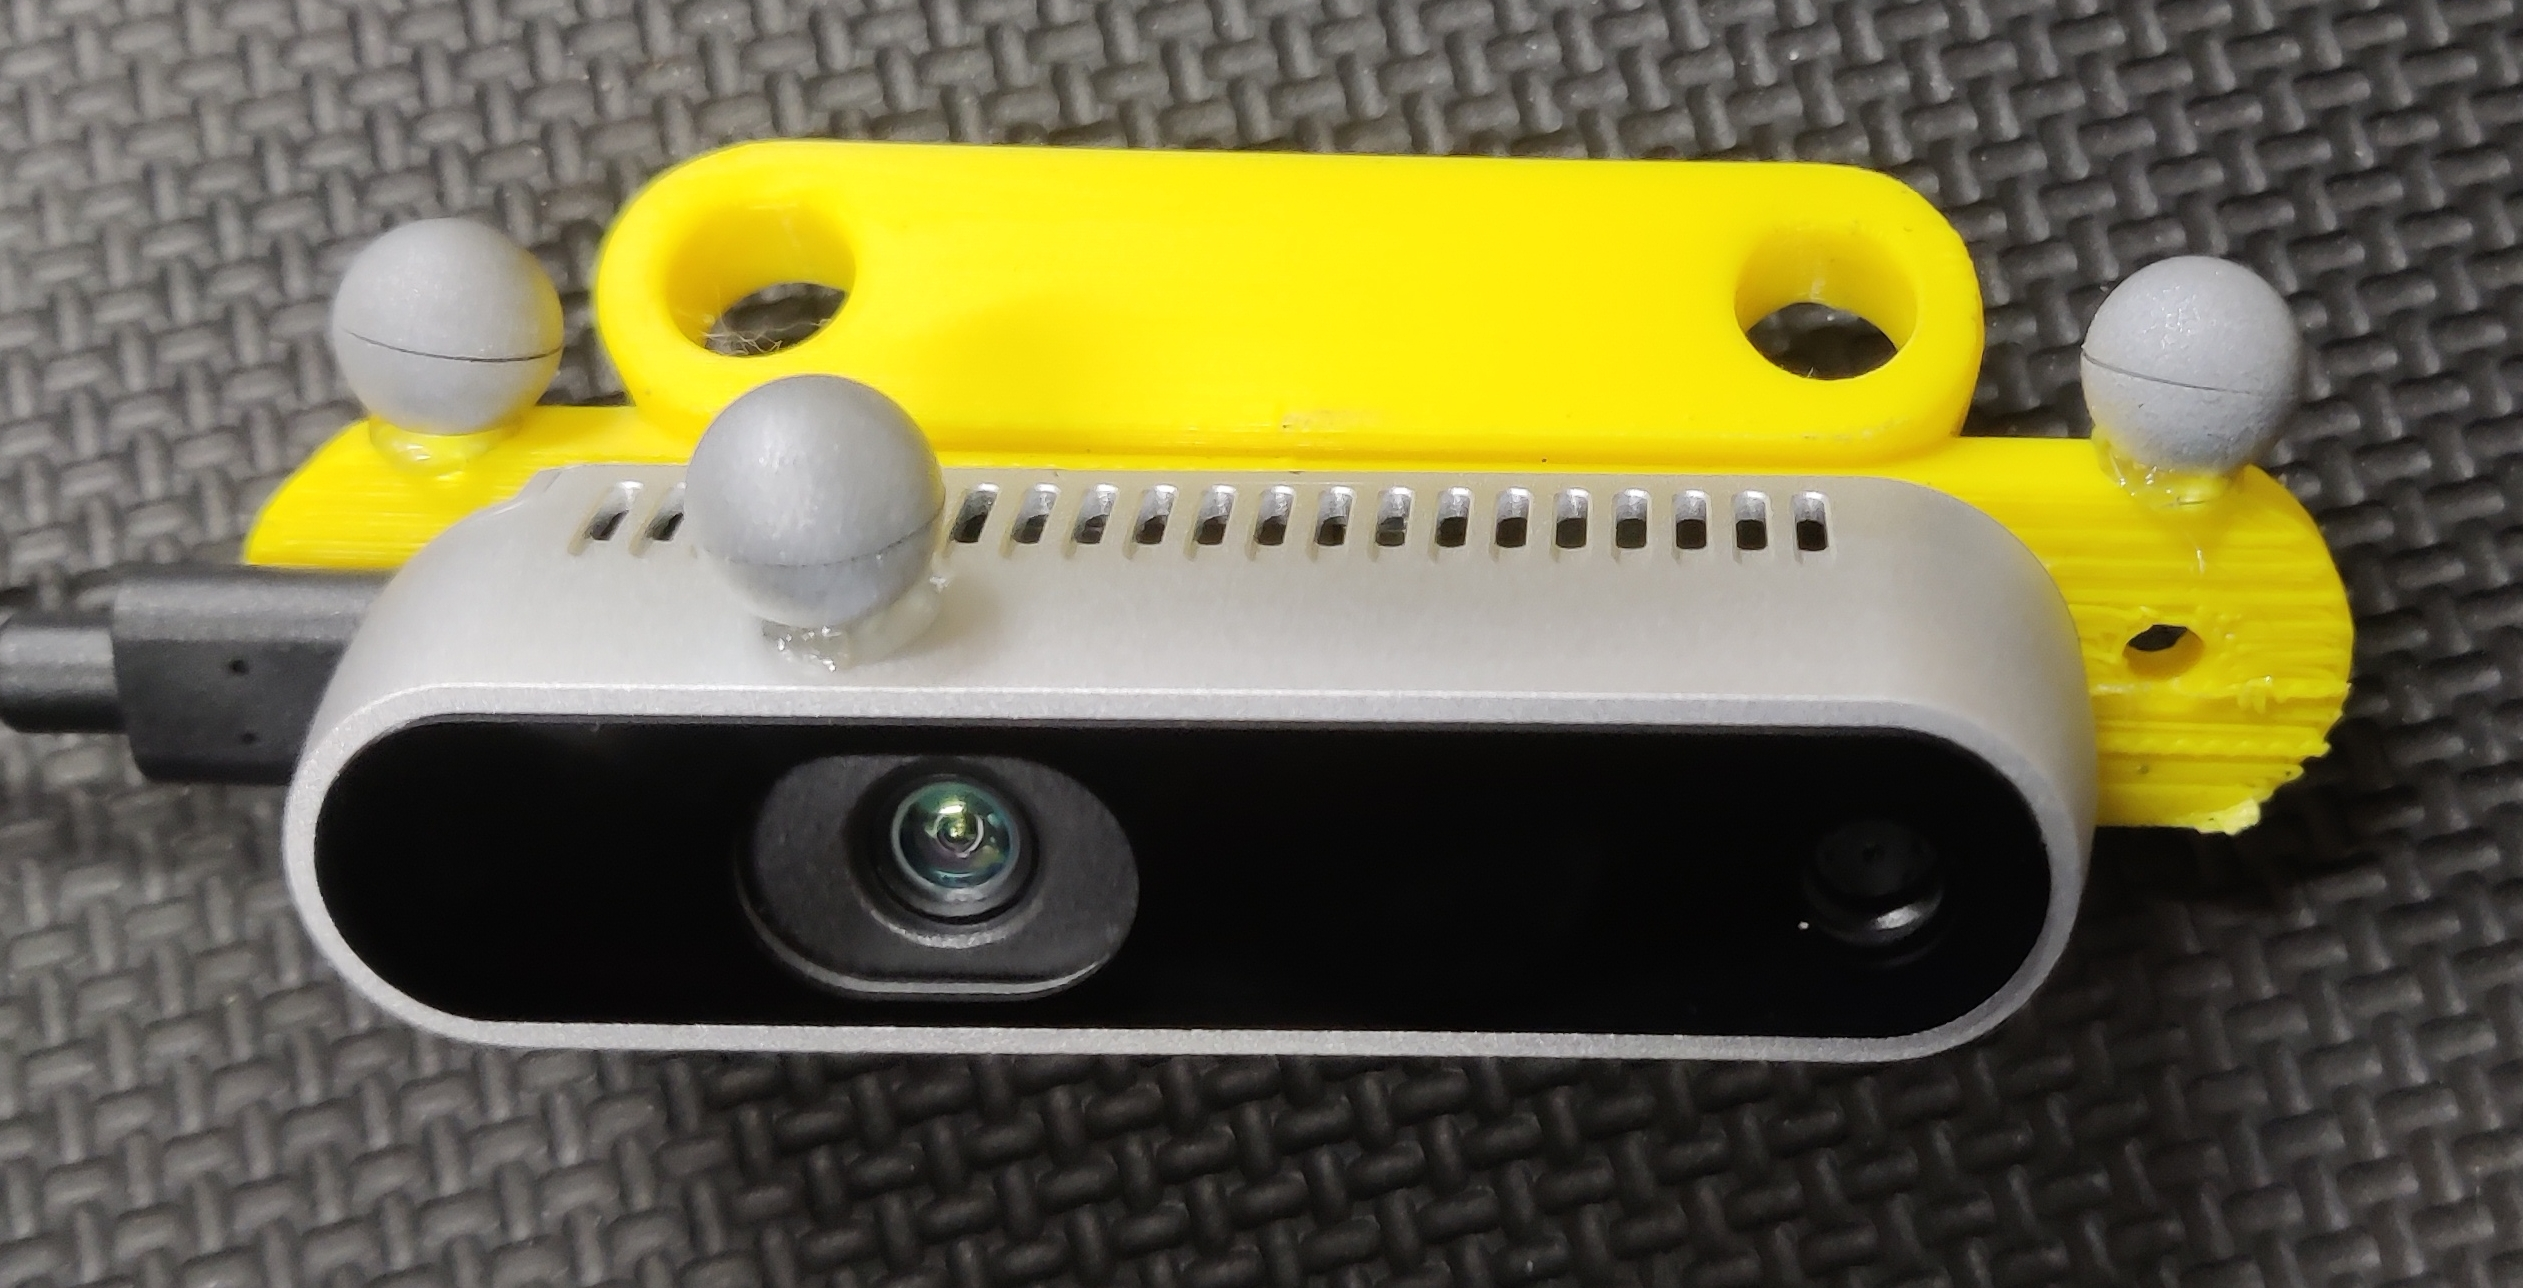
\includegraphics[width=\linewidth]{figures/hardware.jpg}
\hint{RealSense camera with a rigid OptiTrack marker cluster.}
\column{.40\textwidth}
\vspace{.15cm}
\textbf{RGB and depth}\par
30 image pairs per second\par\vspace{.35cm}
\textbf{Gyroscope}\par
200 angular-rate samples per second\par\vspace{.35cm}
\textbf{OptiTrack}\par
120 reference poses per second
\end{columns}
\vspace{.3cm}
Depth gives distance in meters. The gyro measures how fast the camera turns.
\src{Hardware photo: mac\_rgbd\_vio/presentation/figures/rgbd\_cam\_markers.jpg. Stream configuration: enhanced\_live\_vio.py. Motive export header: Take 2026-10-29 08.11.21 PM.csv. Accelerometer packets are recorded but do not drive inertial position integration.}
\end{frame}

% 03 ------------------------------------------------------------------
\begin{frame}[t]{Why errors build up}
\begin{columns}[T,onlytextwidth]
\column{.51\textwidth}
\begin{itemize}\setlength\itemsep{.19cm}
\item A small gyro offset creates tilt over time.
\item Short visual steps can be smaller than measurement noise.
\item A new rotation needs a new translation fit.
\end{itemize}
\vspace{.15cm}
\[\Delta\theta=b_g T\]
{\small $b_g$: constant angular-rate error.\\$T$: time. $\Delta\theta$: accumulated angle error.}
\hint{Example: $0.25^\circ$/s $\times135$ s $=33.75^\circ$.}
\column{.45\textwidth}
\begin{tikzpicture}
\begin{axis}[width=.90\linewidth,height=4.45cm,xlabel={Time (s)},ylabel={Gyro x (rad/s)},xmin=0,xmax=2,scaled y ticks=false,ytick={-.01,-.005,0,.005},legend style={at={(.5,1.03)},anchor=south,legend columns=2},yticklabel style={/pgf/number format/fixed,/pgf/number format/precision=3}]
\addplot[Recorded,thin] table[x=time,y=raw,col sep=comma]{data/gyro_startup.csv};\addlegendentry{Raw}
\addplot[Revised,thin] table[x=time,y=corrected,col sep=comma]{data/gyro_startup.csv};\addlegendentry{Debiased}
\end{axis}
\end{tikzpicture}
\hint{Actual startup samples from the walking capture.}
\end{columns}
\src{Gyro CSV and startup bias from capture\_20261029\_201116. The 0.25 degrees/s illustration is a theoretical constant-bias calculation, not a measured 135-second tilt from this walking take.}
\end{frame}

% 04 ------------------------------------------------------------------
\begin{frame}[t]{Camera motion in one equation}
\vspace{.12cm}
\[\bm P_k=\bm R_{kc}\bm P_c+\bm t_{kc}\]
\vspace{.25cm}
\begin{description}\setlength\itemsep{.17cm}
\item[$\bm P_c,\bm P_k$] The same 3D feature in the current and keyframe cameras, in meters.
\item[$\bm R_{kc}$] A $3\times3$ rotation matrix. It changes the feature's direction.
\item[$\bm t_{kc}$] A 3D translation vector, in meters. It changes the feature's position.
\end{description}
\phys{First rotate a point from the current view into the keyframe view. Then shift it until the two measurements agree.}
\hint{Camera axes: $x$ right, $y$ down, $z$ forward. The world starts at the first camera pose.}
\src{Convention: decoupled\_optimizer.py and pipeline.py. RealSense coordinates: https://github.com/realsenseai/librealsense/blob/master/doc/d435i.md . Initial world Y follows camera Y and is not gravity-calibrated vertical.}
\end{frame}

% 05 ------------------------------------------------------------------
\begin{frame}[t]{Processing steps}
\vspace{.25cm}
\IfFileExists{figures/pipeline.png}{\includegraphics[width=\linewidth,trim=0 140 0 190,clip]{figures/pipeline.png}}{\vspace{3cm}}\par
\vspace{.2cm}
\textbf{Depth supplies metric translation.}\par
The debiased gyro supports rotation between the same image timestamps.
\hint{Concept diagram. All measured results appear later in the presentation.}
\src{Conceptual illustration generated with imagegen for this presentation. Method: enhanced\_vio/src/pipeline.py. Illustration is not an experimental image or numerical evidence.}
\end{frame}

% 06 ------------------------------------------------------------------
\begin{frame}[t]{Gyro bias calibration}
\[\bm b_g=\frac{1}{N}\sum_{j=1}^{N}\bm\omega_{\mathrm{raw},j},\qquad \bm\omega_{\mathrm{corr}}=\bm\omega_{\mathrm{raw}}-\bm b_g\]
\begin{description}\setlength\itemsep{.12cm}
\item[$N$] Number of samples collected while the camera is still.
\item[$\bm b_g$] Mean stationary gyro offset, in rad/s.
\item[$\bm\omega_{\rm raw},\bm\omega_{\rm corr}$] Measured and corrected angular rates, in rad/s.
\end{description}
\phys{Subtract the mean rate measured at rest.}
\vspace{.12cm}
\textbf{Startup:} at least 2 s and 400 samples. Per-axis standard deviation below 0.01 rad/s.\par
\hint{At confirmed stops: $\bm b_g^+=\bm b_g+\alpha(\bar{\bm\omega}_{\rm raw}-\bm b_g)$, with $\alpha=1-e^{-\Delta t/(60\,\mathrm{s})}$. The new bias is $\bm b_g^+$. The bar means interval average. $\Delta t$ is elapsed seconds and $\alpha$ is unitless.}
\src{imu\_calibrator.py. At exactly 200 Hz, 400 samples span 1.995 s, so the duration check normally needs at least 401 samples. Startup also rejects visible motion and a large constant gyro mean. Online updates occur only under the stationary gate.}
\end{frame}

% 07 ------------------------------------------------------------------
\begin{frame}[t]{Gyro rotation between images}
\[\bm R_{\mathrm{imu}}=\prod_j\Exp\!\left(\bar{\bm\omega}_{\mathrm{corr},j}\,\Delta t_j\right)\]
\begin{description}\setlength\itemsep{.18cm}
\item[$\bar{\bm\omega}_{\rm corr,j}$] Mean corrected rate between adjacent IMU samples, in rad/s.
\item[$\Delta t_j$] Actual time between those samples, in seconds.
\item[$\Exp$] Converts an axis--angle vector, in radians, into a 3D rotation matrix.
\item[$\bm R_{\rm imu}$] Current-to-keyframe rotation from the gyro.
\end{description}
\phys{Multiply the small turns in timestamp order to obtain the total rotation.}
\hint{Use camera-frame rates and image timestamps. Vision covers missing IMU intervals.}
\src{gyro\_preintegration.py and pipeline.py. Midpoint rates, image-interval bracketing and actual gyro timestamps. Accelerometer timestamps do not add artificial zero-rate gyro steps.}
\end{frame}

% 08 ------------------------------------------------------------------
\begin{frame}[t]{Stationary gating and zero steps}
\[\begin{aligned}d_{\rm flow}&=\med_i\|\bm u_{c,i}-\bm u_{p,i}\|<0.35\ \mathrm{pixels}\\[4pt]
\max_j\|\bm\omega_{\mathrm{corr},j}\|&<0.025\ \mathrm{rad/s}\end{aligned}\]
{\small $\bm u_p,\bm u_c$: previous and current feature pixels.\\$i$: valid track. $j$: gyro sample in this interval.\par}
\vspace{.15cm}
\textbf{Confirm with at least 20 tracks over three frames.}\par
\vspace{.15cm}
\textbf{Output:} $\Delta\bm p_w=\bm 0$ and $\bm v_w=\bm 0$.\par
\phys{Small image motion and a small turning rate indicate a stop. Hold the current position.}
\hint{$\Delta\bm p_w$: world displacement in meters. $\bm v_w$: velocity in m/s. Keep the existing keyframe offset to avoid a backward jump.}
\src{zupt\_detector.py and pipeline.py. Flow is previous-frame-to-current-frame displacement, not keyframe disparity. Maximum corrected gyro norm prevents opposing turns from canceling. This is a gate, not a Kalman velocity-state update.}
\end{frame}

% 09 ------------------------------------------------------------------
\begin{frame}[t]{Keyframes give a larger visual baseline}
\begin{columns}[T,onlytextwidth]
\column{.66\textwidth}
\vspace{.1cm}
\IfFileExists{figures/keyframes.png}{\includegraphics[width=\linewidth,height=4.75cm,keepaspectratio]{figures/keyframes.png}}{\vspace{3cm}}
\column{.30\textwidth}
\textbf{New keyframe if any condition holds}\par\vspace{.25cm}
Median disparity $>3.5$ px\par\vspace{.25cm}
Relative turn $>2.5^\circ$\par\vspace{.25cm}
Inliers $<65\%$ of reference points
\end{columns}
\phys{A fixed reference lets visual motion grow above the noise.}
\hint{Disparity is keyframe-to-current pixel motion. Inliers agree with the 3D motion fit.}
\src{keyframe\_tracker.py. Generated schematic, not a measured 4x to 8x SNR claim. Thresholds can still insert keyframes frequently. Supported tracks can be reused, with detection when their count falls.}
\end{frame}

% 10 ------------------------------------------------------------------
\begin{frame}[t]{Depth turns image pixels into 3D points}
\[\bm P=d\begin{bmatrix}(u-c_x)/f_x\\[2pt](v-c_y)/f_y\\[2pt]1\end{bmatrix}\]
\begin{description}\setlength\itemsep{.14cm}
\item[$u,v$] Feature position in the image, in pixels.
\item[$c_x,c_y$] Camera image center, in pixels.
\item[$f_x,f_y$] Camera focal lengths, in pixels.
\item[$d,\bm P$] Depth and the resulting 3D point, in meters.
\end{description}
\phys{The pixel gives direction. Depth gives distance along that direction.}
\hint{At 2 m depth, one pixel represents about 3.3 mm when $f_x\simeq607$ px.}
\src{calibrated\_covariance.py and keyframe\_tracker.py. Pinhole unprojection uses aligned RGB-depth and color intrinsics. The pixel example holds depth fixed and is illustrative.}
\end{frame}

% 11 ------------------------------------------------------------------
\begin{frame}[t]{Uncertainty sets the weight of each match}
\[\bm\Sigma_{3D}=\bm J\bm\Sigma_m\bm J^T\]
\[\bm\Sigma_r=\bm\Sigma_k+\bm R\bm\Sigma_c\bm R^T,\qquad \bm\Omega=\bm\Sigma_r^{-1}\]
\begin{description}\setlength\itemsep{.11cm}
\item[$\bm\Sigma_m,\bm J$] Pixel/depth uncertainty and its conversion to 3D.
\item[$\bm\Sigma_k,\bm\Sigma_c$] Keyframe/current 3D covariances, in m$^2$.
\item[$\bm\Sigma_r,\bm\Omega$] Match covariance in m$^2$ and inverse covariance in m$^{-2}$.
\end{description}
\phys{Uncertain directions receive less weight. Combine both covariances in the same frame.}
\hint{$\bm J$ carries the conversion from pixels and depth into 3D position errors.}
\src{Inherited parameters: config/optitrack\_calibrated\_covariance.yaml. calibrated\_covariance.py and DecoupledOptimizer.information. Measurement covariance has mixed pixel-squared and meter-squared units; J converts them. No new held-out covariance calibration was established.}
\end{frame}

% 12 ------------------------------------------------------------------
\begin{frame}[t]{Stage 1: rotation fusion}
\[\bm\phi_f=0.75\Log(\bm R_{\rm vis})+0.25\Log(\bm R_{\rm imu})\]
\[\bm R^*=\Exp(\bm\phi_f)\]
\begin{description}\setlength\itemsep{.14cm}
\item[$\bm R_{\rm vis}$] Rotation fitted from matched 3D points.
\item[$\bm R_{\rm imu}$] Debiased gyro rotation over the same time interval.
\item[$\Log,\bm\phi_f$] Matrix-to-axis--angle map and the fused angle vector, in radians.
\end{description}
\phys{Average small rotation vectors, then convert the result to a valid rotation matrix.}
\hint{The fixed 75/25 split is a design choice. $\bm\phi_f$ is an angle, not a rate.}
\src{decoupled\_optimizer.py. Visual fit uses RANSAC and robust metric refinement. Both rotations map current coordinates into the same keyframe coordinates. This tangent-space blend is a local small-rotation rule.}
\end{frame}

% 13 ------------------------------------------------------------------
\begin{frame}[t]{Stage 2: translation with rotation fixed}
\[\bm d_i=\bm P_{k,i}-\bm R^*\bm P_{c,i}\]
\[\bm t^*=\left(\sum_i w_i\bm\Omega_i\right)^{-1}\sum_i w_i\bm\Omega_i\bm d_i\]
\begin{description}\setlength\itemsep{.12cm}
\item[$\bm d_i$] Shift suggested by match $i$, in meters, after the fused rotation.
\item[$w_i,\bm\Omega_i$] Unitless outlier weight and information matrix in m$^{-2}$.
\item[$\bm t^*$] Weighted best translation, in meters.
\end{description}
\phys{With the turn fixed, choose the shift that best aligns the points.}
\hint{Huber weights reduce outlier influence. Repeat the exact weighted solve until stable.}
\src{DecoupledOptimizer.solve\_translation. Huber weight decreases with large Mahalanobis residual. Conditional weighted least-squares, not a one-shot robust closed form. Translation is always refitted after rotation fusion.}
\end{frame}

% 14 ------------------------------------------------------------------
\begin{frame}[t]{A reference pose anchors the world position}
\[\bm R_{wc}=\bm R_{wk}\bm R_{kc}\]
\[\bm p_{wc}=\bm p_{wk}+\bm R_{wk}\bm t_{kc}\]
\begin{description}\setlength\itemsep{.14cm}
\item[$\bm R_{wk},\bm p_{wk}$] Keyframe orientation and position in the world.
\item[$\bm R_{kc},\bm t_{kc}$] Current camera pose relative to that keyframe.
\item[$\bm R_{wc},\bm p_{wc}$] Current camera orientation and position in the world.
\end{description}
\phys{Rotate the local translation into the world. Then add it to the fixed keyframe position. All position vectors use meters.}
\hint{Anchor each pose to its keyframe. Never add the full relative offset twice.}
\src{pipeline.py. Camera poses map to initial-camera world. A stationary gate holds world position and zeros finite-difference velocity. Loss holds the last reliable pose, so motion through loss remains unknown.}
\end{frame}

% 15 ------------------------------------------------------------------
\begin{frame}[t]{CPU work and recording}
\begin{columns}[T,onlytextwidth]
\column{.52\textwidth}
\begin{tikzpicture}
\begin{axis}[width=.95\linewidth,height=4.9cm,ybar,bar width=13pt,ymin=0,ymax=64,ylabel={Estimator time (ms)},xtick={1,2},xticklabels={Live,Replay},legend style={at={(.5,1.03)},anchor=south,legend columns=2},nodes near coords,every node near coord/.append style={font=\scriptsize,/pgf/number format/fixed,/pgf/number format/precision=1}]
\addplot[fill=Teal!80,draw=none] table[x=run,y=mean,col sep=comma]{data/timing.csv};\addlegendentry{Mean}
\addplot[fill=Navy!65,draw=none] table[x=run,y=p95,col sep=comma]{data/timing.csv};\addlegendentry{95th percentile}
\end{axis}
\end{tikzpicture}
\column{.43\textwidth}
\textbf{Less repeated work}\par
Batch RANSAC hypotheses.\par
Compute uncertainty at feature locations.\par\vspace{.3cm}
\textbf{Separate file writing}\par
Background workers save raw data.\par
Explicit counters report lost frames.
\end{columns}
\hint{Replay timing is offline. It does not establish 30 FPS during live walking. All estimator computation uses the CPU.}
\src{Walking live timing: mean 39.7764 ms, p95 53.9299 ms. Final replay: mean 18.1682 ms, p95 24.5360 ms. Revision uses 300 features, four OpenCV threads and a 15 Hz HUD. Original capture lost 1,065 frames, which saved images cannot reconstruct.}
\end{frame}

% 16 ------------------------------------------------------------------
\begin{frame}[t]{Clock synchronization with independent gyro data}
\begin{columns}[T,onlytextwidth]
\column{.38\textwidth}
\[t_{\rm GT}=t_{\rm camera}+\tau\]
{\small $t$: time in seconds.\\$\tau$: clock offset in seconds.}\par\vspace{.28cm}
Compare raw gyro turning with OptiTrack orientation changes.\par\vspace{.25cm}
\textbf{Correlation: 0.912}\par
40.58 s of reliable support
\column{.58\textwidth}
\begin{tikzpicture}
\begin{axis}[width=\linewidth,height=4.9cm,xlabel={OptiTrack time (s)},ylabel={Angular speed (rad/s)},xmin=0,xmax=85,ymin=0,ymax=1.5,legend style={at={(.5,1.03)},anchor=south,legend columns=2}]
\addplot[Teal,thin] table[x=time,y=speed,col sep=comma]{data/gyro_sync.csv};\addlegendentry{Gyro}
\addplot[Recorded,thin] table[x=time,y=speed,col sep=comma]{data/gt_sync.csv};\addlegendentry{OptiTrack}
\end{axis}
\end{tikzpicture}
\end{columns}
\hint{Use 0.3 s orientation windows to reduce noisy derivatives. No position error is used to choose the time shift.}
\src{synchronize\_walking\_run.py and imu\_sync/synchronization.json. Shift from first gyro packet: -4.71 s. Absolute shift: -1793284882.0330672 s because clocks have different origins. Support excludes long GT gaps and implausible orientation flips. GT positions remain unchanged.}
\end{frame}

% 17 ------------------------------------------------------------------
\begin{frame}[t]{Accuracy measurement}
\[\mathrm{ATE}_{\rm RMSE}=\sqrt{\frac{1}{M}\sum_{i=1}^{M}\left\|\bm R_a\bm p_i^{\rm est}+\bm t_a-\bm p_i^{\rm GT}\right\|^2}\]
\begin{description}\setlength\itemsep{.12cm}
\item[$M$] Number of valid, time-matched position pairs.
\item[$\bm R_a,\bm t_a$] One rigid coordinate alignment. Scale stays equal to one.
\item[$\bm p^{\rm est},\bm p^{\rm GT}$] Estimated and reference positions, in meters.
\end{description}
\phys{ATE measures typical position error after rigid alignment, in meters.}
\vspace{.15cm}
\textbf{902 matched poses cover 63.7\% of the recorded trajectory.}
\hint{Exclude GT gaps above 0.1 s. This take has 105 such gaps, up to 2.84 s long.}
\src{comparison/benchmark\_metrics.json. Separate Umeyama rigid alignment per estimate, same GT times. Only 5,126 of 11,527 rows contain valid rigid-body poses. Marker-to-camera lever arm was not supplied. ATE/path is normalized ATE, not endpoint drift.}
\end{frame}

% 18 ------------------------------------------------------------------
\begin{frame}[t]{Walking trajectory on valid reference intervals}
\begin{columns}[T,onlytextwidth]
\column{.63\textwidth}
\begin{tikzpicture}
\begin{axis}[width=\linewidth,height=5.35cm,axis equal image,xlabel={$X$ (m)},ylabel={$Z$ (m)},legend style={at={(.02,.02)},anchor=south west},xmin=-2,xmax=1.8,ymin=-1.6,ymax=1.9]
\addplot[black,dashed,line width=.9pt] table[x=x,y=z,col sep=comma]{data/gt.csv};\addlegendentry{OptiTrack}
\addplot[Recorded,line width=.7pt] table[x=x,y=z,col sep=comma]{data/recorded.csv};\addlegendentry{As recorded}
\addplot[Revised,line width=.7pt] table[x=x,y=z,col sep=comma]{data/revised.csv};\addlegendentry{Revision replay}
\end{axis}
\end{tikzpicture}
\column{.32\textwidth}
\vspace{.35cm}
{\color{Recorded}\Large\bfseries 0.420 m}\par Recorded ATE\par\vspace{.45cm}
{\color{Revised}\Large\bfseries 0.308 m}\par Revised replay ATE\par\vspace{.4cm}
About 27\% lower ATE on this valid subset.
\end{columns}
\hint{The figure breaks lines across missing GT. This take also served to validate the revision, so it is not an independent held-out test.}
\src{comparison/aligned\_comparison.npz and benchmark\_metrics.json. Same 902 poses, scale one. This is a new take, not the historical 135-second take with 1.616 m ATE. Do not present these as a direct old-take before/after.}
\end{frame}

% 19 ------------------------------------------------------------------
\begin{frame}[t]{Path inflation and vertical error remain}
\begin{columns}[T,onlytextwidth]
\column{.49\textwidth}
\begin{tikzpicture}
\begin{axis}[width=\linewidth,height=4.45cm,ybar,bar width=23pt,title={Path on matched timestamps},ylabel={Path length (m)},ymin=0,ymax=33,xtick={1,2,3},xticklabels={GT,Recorded,Replay},nodes near coords,every node near coord/.append style={font=\small,/pgf/number format/fixed,/pgf/number format/precision=2}]
\addplot[fill=Teal!75,draw=none] table[x=run,y=path,col sep=comma]{data/path.csv};
\end{axis}
\end{tikzpicture}
\column{.49\textwidth}
\begin{tikzpicture}
\begin{axis}[width=\linewidth,height=4.45cm,ybar,bar width=23pt,title={Vertical-error change},ylabel={Absolute change (m)},ymin=0,ymax=.55,xtick={1,2},xticklabels={Recorded,Replay},nodes near coords,every node near coord/.append style={font=\small,/pgf/number format/fixed,/pgf/number format/precision=3}]
\addplot[fill=Recorded!80,draw=none] table[x=run,y=error,col sep=comma]{data/vertical.csv};
\addplot[black,dashed,sharp plot,domain=.5:2.5,samples=2,nodes near coords={}] {.25};
\end{axis}
\end{tikzpicture}
\end{columns}
\textbf{Tracking failures: 58 recorded, 66 in the revised replay.}
\hint{Dashed line: 0.25 m target. Vertical change uses aligned OptiTrack $Y$ between evaluated endpoints. Paths bridge excluded intervals.}
\src{comparison/benchmark\_metrics.json. Common paths: 14.3232, 25.6703, 27.1066 m. Absolute vertical-error changes: 0.445763, 0.284475 m. Peak-to-peak errors: 1.0574 and 0.9628 m. The previous take's 34.5 m path target does not apply here.}
\end{frame}

% 20 ------------------------------------------------------------------
\begin{frame}[t]{What the evidence supports}
\vspace{.12cm}
\textbf{Established on this capture}\par\vspace{.15cm}
The revised replay reduces ATE and estimator CPU time.\par
Twenty numerical and integration tests pass.\par
\vspace{.45cm}
\textbf{Still unresolved}\par\vspace{.15cm}
Path inflation, motion through tracking loss, and vertical error.\par
Zero-drop 30 FPS during a new live walking trial.\par
\vspace{.45cm}
\textbf{Next measurements}\par\vspace{.15cm}
Improve marker visibility and measure the marker-to-camera offset.\par
Run repeated walking trials with matched OptiTrack recordings.
\hint{A short updated stationary live check reached 29.87 FPS with five acquisition drops. It does not establish 30 FPS during walking.}
\src{walking\_201116/REPORT.md, tests.txt, verification.json and live\_revision\_check/timing.json. Twenty-one original source files remain unchanged. Future work needs held-out trials, independent synchronization and ablations. Hardware: https://github.com/realsenseai/librealsense/blob/master/doc/d435i.md . Point covariance context: https://isprs-annals.copernicus.org/articles/II-5-W2/127/2013/ .}
\end{frame}
\end{document}
